\begin{exercises}
\emph{In problems 1--28, let $U=\{1,2,3,\ldots,10\}$, $A=\{1,3,5,7\}$, $B=\{1,2,3,4\}$, and $C=\{3,4,6,7,9\}$.\\ Find each of the following sets.}

\pfour{$A^c$}
\pfour{$B^c$}
\pfour{$A \cup C$}
\pfour{$A \cap B$}

\pfour{$B \cap C$}
\pfour{$A \cup B$}
\pfour{$A \setminus B$}
\pfour{$C \setminus A$}

\pfour{$A^c \cap B^c$}
\pfour{$A^c \cup C$}
\pfour{$B \cup C^c$}
\pfour{$A \cap B^c$}

\pfour{$(A \cup C^c)^c$}
\pfour{$(B^c \cap C)^c$}
\pfour{$(A \cap B)^c$}
\pfour{$(B \cup A)^c$}

\pfour{$A \cup \varnothing$}
\pfour{$B \cup \varnothing$}
\pfour{$C \cup \varnothing$}
\pfour{$B \cap \varnothing$}

\pfour{$(A \cap B) \cup C$}
\pfour{$(A \cup C) \cap B$}
\pfour{$B \cup (A \cap C)$}
\pfour{$(A \cap B) \cup (C \cap B)$}

\pfour{$(B \cup A) \cap (B \cup C)$}
\pfour{$(A \cup C)^c \cap B^c$}
\pfour{$A \cap B \cap C$}
\pfour{$A \cup B \cup C$}

\emph{In problems 29--40, use the following Venn diagram to find each set.}
\begin{center}
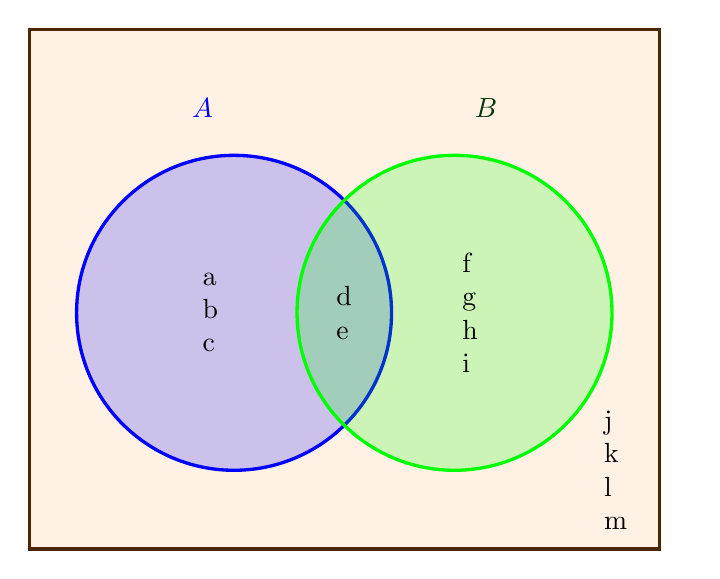
\begin{tikzpicture}
  \draw [very thick,color=orange!30!black, fill=orange, fill opacity=0.1] (-4cm,-3cm) rectangle (4cm,3.6cm);

  \draw [very thick,color=blue, fill=blue, fill opacity=0.2] (-1.4,0) circle (2cm);
  \draw [very thick,color=green, fill=green, fill opacity=0.2] (1.4,0) circle (2cm);
  \draw [yshift=2.6cm,xshift=-1.8cm] node {\color{blue} $A$};
  \draw [yshift=2.6cm,xshift=1.8cm] node {\color{green!20!black} $B$};
  
  \draw [yshift=0cm,xshift=-1.3cm] node {\parbox{1cm}{a\\b\\c}};
  \draw [yshift=0cm,xshift=2cm] node {\parbox{1cm}{f\\g\\h\\i}};
  \draw [yshift=0cm,xshift=0.4cm] node {\parbox{1cm}{d\\e}};
  \draw [yshift=-2cm,xshift=3.8cm] node {\parbox{1cm}{j\\k\\l\\m}};
  
\end{tikzpicture}
\end{center}

\pfour{$A^c$}
\pfour{$A \cup B$}
\pfour{$(A \cap B)^c$}
\pfour{$A^c \cup B^c$}

\pfour{$A \setminus B$}
\pfour{$B \setminus A$}
\pfour{$A^c \cap B^c$}
\pfour{$(A \cup B)^c$}

\pfour{$U$}
\pfour{$A^c \cup B$}
\pfour{$A \cap B^c$}
\pfour{$A \setminus U$}
\end{exercises}